\chapter{Introduction}%
\label{chap:introduction}
\textit{This chapter narrows the broad field of robotics down to a largely unsolved problem. For that problem the state of the art methods are presented, and their shortcomings are highlighted. \Cref{sec:research_question} addresses the current gap in research with the main and sub research questions. A largely unsolved problem is then narrowed down to the scope of this thesis in problem description,~\cref{sec:problem_description}. The chapter finishes by presenting all upcoming chapters in the report structure,~\cref{sec:report_structure}.\bs}

\todo[inline]{Corrado: All my feedback latest feedback from this chapter}
\todo[inline]{Martijn: these paragraphs are hard to read, because they appear like separate summaries of work from literature, rather than parts of a coherent story line. The first and last sentences of paragraphs are crucial for improving this.}

% introduce 3 topics that arise for robots in new environments. Explain the arisen problem, and the 2 main approaches toward solving that problem. 
For robots, it remains a hard problem to navigate and act in new, unseen environments. It can be motivated that this is due to many challenges that the robot has to overcome. In this thesis such challenges are categorised into 3 topics, namely: \textbf{\ac{NAMO}}, \textbf{nonprehensile manipulation planning}, and \textbf{learning object dynamics}. Robots face unseen environments during space exploration, rescue missions in collapsed buildings. New environments can also emerge from familiar but changed environments, for example a warehouse in which a fallen package leaked fluids over the floor. Learning abilities improve robots to adapt to environmental changes. Research into approaches tackling the 3 topics just described can be split into two categories. The bulk falls into hierarchical approaches~\cite{kaelbling_hierarchical_2011,scholz_navigation_2016,krontiris_dealing_2015}. A hierarchical structure generally consists of a high-level and a low-level component. The high-level task planner has an extended time horizon which includes several atomic actions and their sequencing. Whilst a low level controller acts to accomplish a single action (e.g.~drive toward object, push object, drive toward target location are 3 single actions), by sending input signals toward the robot actuators. The high-level planner has a prediction horizon consisting of an action sequence, a long prediction horizon compared to the low-level planner whose prediction horizon is maximal for a single action. Hierarchical structures generally provide solutions which are computationally efficient but are hierarchical, meaning the solutions found are the best feasible solutions in the task hierarchy they search. The quality of the solution depends on the hierarchy which is typically hand-coded and domain-specific~\cite {vega-brown_asymptotically_2020}. 

\todo[inline]{explain searching the joint config space without mentioning the joint config space}
Alternatively to hierarchical approaches, solutions can be provided by searching in a joint configuration space of the robot and objects, where the robots configuration space is augmented with environment objects configuration spaces whilst also including dynamic constraints~\cite{hauser_multimodal_2010,berenson_manipulation_2009,jaillet_path_2013}. Such a joint configuration space suffers from a combinatorial explosion and it is practically 
\todo[inline]{Corrado:So far it was pretty general but now you talk about configuration space of objects and robot. What is the message you want to pass to the reader in this paragraph? Make it clear }
\todo[inline]{Martijn: not impossible; there are many papers showing how to do it. Be more precise in your statement.}impossible to find a path connecting a start to the target configuration. Because an action sequence from searching in a joint configuration is exhaustive,

\todo[inline]{Martijn: Sentence structure is incorrect, because it is not the "action sequence" that is exhaustivecu} 

simplifications are leveraged. For example, a search close to the current configuration, lets the robot track this incomplete solution toward a desired goal. Alternation between searching the joint configuration space and tracking the incomplete solution results in converging toward the desired point in the joint configuration space. \todo[inline]{martijn: this is a very generic and uninformative statement. At least provide a reference to a survey paper that lists these techniques. Preferably, you list the main categories of solutions here in this sentence (still including references).}
Different techniques exist to prevent searching in the entire joint configuration space.\bs

\todo[inline]{Martijn: I don't like this informal writing style. About: evironments is a broad topic, let’s narrow down the scop}
In the scope of this thesis, we consider a challenging and largely unsolved problem of navigation among movable objects in unknown environments. Consider a simple robot without grippers or arms attached in an environment with movable objects. The environment consists of a flat ground plane, the robot and movable objects. By driving against objects the robot can manipulate objects.\bs
\todo[inline]{Corrado: A paragraph is used to split different part of the narrative, not connected concepts like this ones Gijs: do not split that stuff}
\todo[inline]{Martijn: It is good that you narrow down the scope here. However, your reader will wonder why you narrowed it down in this specific way, what is the reasoning?}
This creates two different modes of dynamics (driving,  pushing) where different differential constraints apply to the different modes. Because there is a discontinuity in the constraints the joint configuration space is a piecewise-analytic configuration space, which complicates motion planning considerably~\cite{vega-brown_asymptotically_2020}. Whilst the robot can interact with the objects in the environment, there is no prior information provided to the robot (e.g. weight, friction coefficient) other than the shape and pose of the object. By interacting with objects, the robot can generate a system model, describing the expected trajectory of an object as a result of a push from the robot. The robot is tasked to relocate a subset of objects by pushing objects. \bs


\todo[inline]{Martijn: "lesser researched" doesn't sound like proper Englishkj}

The domain just described is (partially) the subject of three different areas of research, namely \textbf{\ac{NAMO}}, \textbf{nonprehensile manipulation planning}, and \textbf{learning object dynamics}. Individually a considerable amount of research is done on these topics (\ac{NAMO}~\cite{wang_affordancebased_2020,lavalle_planning_2006,elbanhawi_samplingbased_2014,kingston_samplingbased_2018,chen_fast_2018,ellis_navigation_2022}, nonprehensile manipulation planning~\cite{arruda_uncertainty_2017,mericli_pushmanipulation_2015,toussaint_sequenceofconstraints_2022,stuber_let_2020,stuber_featurebased_2018,bauza_dataefficient_2018}, learning object dynamics~\cite{seegmiller_vehicle_2013,cong_selfadapting_2020}), combining two topics recieves little attention by scientific community, and combining all three topics even scarcer.\bs

\todo[inline]{Martijn: This paragraph doesn't seem to add much real information, feels more like some random thoughts that happened to come up at some point.}
Combining learning, driving and pushing can improve the driving and pushing skills of the robot. Learning is crucial for unforeseen environments, for example during space exploration. Non-prehensile pushing compared to prehensile pushing saves weight, and for a robot with a gripper the ability for nonprehensile pushing comes in handy when the gripper is already in use, for example when a robot relocates a package with its gripper, it encounters a blocked path by an unknown object. Blocked paths and changing environments often coincide, such as a fallen package in a warehouse spilling fluid on the floor, with learning the robot can account for the slippery floor. Finally learning may improve single actions, but it may also improve long-term action planning.\bs
\todo[inline]{MARTIJN: it is strange to talk about a gripper here, while you already narrowed down the scope to non-gripper robots two paragraphs above.k}

\citeauthor{vega-brown_asymptotically_2020} investigated \ac{NAMO} in a piecewise-analytic configuration space to relocate objects~\cite{vega-brown_asymptotically_2020}. Whilst an optimal plan is obtained with probability one with infinite samples, the algorithm does not learn the pushing relation between the robot and the objects. The ability to learn push dynamics greatly broadens the variety of objects a robot can push. Realistically, robots in warehouses, hospitals or supermarkets might encounter a variety of different objects, but learning dynamics inevitably leads to system model mismatch. A motion planning algorithm should be compatible with learned system models and take model mismatch into account. Learning dynamics is a topic untouched by \citeauthor{vega-brown_asymptotically_2020} because the robot can rigidly grasp the box so that the robot-box pair behaves as a single rigid body as long as the box is grasped. This model avoids the complexity of real-world pushes, becoming alienated from reality.\bs

\citeauthor{wang_affordancebased_2020} takes nonprehensile manipulation planning out of the equation and only focuses on the \ac{NAMO} problem and learning system dynamics. Learning interaction by embedding unknown objects with affordance information followed by planning with a contact-implicit motion planner toward a robot goal location~\cite{wang_affordancebased_2020}. By removing push manipulation, finding a path from a start to target configuration simplifies, only a single mode of dynamics is contained in the configuration space and the piecewise-analytic configuration space becomes a configuration space. There exist a variety of sampling-based motion planners that can find a path with properties such as probabilistic completeness, replanning in dynamic environments, planning under uncertainty or asymptotically optimality~\cite{karaman_samplingbased_2011,elbanhawi_samplingbased_2014}. Challenging problems introduced by push manipulation are removed by simply removing push manipulation.\bs

\citeauthor{vega-brown_asymptotically_2020} combined \ac{NAMO} with nonprehensile manipulation panning, \citeauthor{wang_affordancebased_2020} combines \ac{NAMO} with learning system models. Both combine 2 of the 3 topics allowing for a more in-depth analysis but avoiding the problems introduced by combining all 3 topics (\ac{NAMO}, nonprehensile manipulation planning and learning system models). \citeauthor{sabbaghnovin_model_2021} does combine all three topics. She proposes to obtain system models by analysing and converting a limited set of robot-object test pushes using Bayesian regression to predict model parameters. Path planning is the result of solving a proposed mixed-integer convex optimization~\cite{sabbaghnovin_optimal_2016} which is tracked by \ac{MPC} control, the proposed method is tested in a hospital setting~\cite{novin_dynamic_2018} and was later improved upon resulting in lowering trajectory errors~\cite{sabbaghnovin_model_2021}.\bs

\todo[inline]{Martijn: with this (and the previous) paragraph, I wonder: what is your point?}

Since \citeauthor{sabbaghnovin_model_2021} uses a gripper to manipulate objects, the research falls into the category of prehensile manipulation. Prehensile manipulation in comparison with nonprehensile manipulation is simpler because a pushed object becomes disconnected easier compared to a gripped object. Her research is specific to legged objects, which limits the set of objects to manipulate considerably.\bs

This thesis proposes a method where the robot should learn robot and object dynamics by interaction, and perform motion and manipulation planning whilst facing a wide variety of objects, tasks and environments. The 3 topics (\ac{NAMO}, nonprehensile manipulation planning and learning system models) are bundled together with a technique known as \textbf{backward induction} also known as \textbf{backward tracing} or \textbf{backward search} (this thesis will refer to this technique with the term backward search).\todo[inline]{Marijn: strange sentence} The proposed method in this thesis and \citeauthor{sabbaghnovin_model_2021} proposed method solve comparable problems using different techniques, allowing for easy comparison between the results of \citeauthor{sabbaghnovin_model_2021} and the results from the proposed method in this thesis.\bs
\todo[inline]{Martijn : explain backward induction, backward tracing and provide references}

\section{Research Question}%
\label{sec:research_question}
To investigate the effect of learning on action selection and on action planning the following research questions have been selected.\bs

\textbf{Main research question:}
\begin{center}%
\label{researchquestion:main}
\large
How do learned objects' system models improve global task planning\\for a robot with nonprehensible manipulation abilities over time?
\end{center} 

The main research question is split into two smaller more detailed subquestions. Essentially the first research subquestion asks \quotes{how does the proposed method work?}, which allows to explain the proposed method. The second research subquestion essentially asks: \quotes{How does it compare to similar existing methods?}, allowing to compare the proposed methods with existing state-of-the-art methods by comparing their results.\bs

\textbf{Research subquestion:}
\begin{enumerate}
    \item\label{researchsubquestion:does_it_work} Can the proposed method combine learning and planning for push en drive applications with a technique known as backward search~\cite{krontiris_dealing_2015}?
    \item\label{researchsubquestion:does_it_compare} How does learning system models and remembering interactions compare to only learning system models? And, how does the proposed method compare against the state of the art? 
\end{enumerate}

Answering the research subquestions provides a solid base to answer the main research question. The main research question is aimed to test robot abilities in a new environment, and track improvement in that a new environment. Some questions which come up are: Will the robot prefer specific strategies for certain objects? How much improvement will a robot make with some experience? Will the robot converge to a preferred strategy for an object, and will it converge to the same strategy again if its memory is wiped.\bs

\section{Problem Description}%
\label{sec:problem_description}
\todo[inline]{Martijn: So, why at all was a 3D environment selected?}
To answer the research questions, tests will be performed in a robot environment. A simple environment is desired because that will simplify testing, yet the robot environment should represent many real-world environments in which robots operate. For the environment, a flat ground plane is selected, since many mobile robots operate in a workspace with a flat floor, such as a supermarket, warehouse or distribution centre. The robots to test should be flat robots, which lowers the chance of tipping over. A 3-dimensional environment is selected, but with a flat floor and a flat robot can be treated as a 2-dimensional problem because the robot and objects can only change position over $x$ and $y$ axis ($xy$ plane parallel to the ground plane) and rotate around the $z$ axis (perpendicular to the ground plane).\bs

Let's start with defining the environment.\\Let the tuple $\left\langle \text{Origin}, \text{Ground Plane}, \text{Ob}, E \right\rangle$ fully define a robot environment where:\bs

\par\smallskip\noindent
\centerline{\begin{minipage}{0.8\textwidth}
\begin{enumerate}
  \item[Origin] Static point in the environment with a $x$-, $y$- and $z$-axis. Any point in the environment has a linear and an angular position and velocity with respect to the origin \vspace{0.5\baselineskip}
 \item[Ground Plane] A flat plane parallel with the Origin's $x$- and $y$- axis. Objects cannot pass through the ground plane and meet sliding friction when sliding over the ground plane. \vspace{0.5\baselineskip}
 \item[Ob] A set of objects, $\text{Ob} = (obst_1, obst_2, obst_3, \dots, obst_i)$ with $i>1$, an object is a 3-dimensional body with shape and uniformly distributed mass. Examples of objects are given in \cref{fig:example_objects}. \vspace{0.5\baselineskip}
  \item[$E$] A set of motion equations describing the behaviour of objects such as gravity, interaction with the ground plane or interaction with other objects. The motion equations are equivalent to the true dynamics. \vspace{0.5\baselineskip}
\end{enumerate}
\end{minipage}}
\par\smallskip

   \todo[inline]{Martijn: Why do you call them "obst"? This seems related to the woord Obstacle, not Object.}
   \todo[inline]{Marijn: why do you say i>1?}

\todo[inline]{Martijn: what does this mean, "equivalent to the true dynamics"?}
A state consists of the linear and angular position and velocity of a point with respect to the environment's origin.\bs
\todo[inline]{Martijn: points cannot have angular positions. Also, I don't think that states are properties of points, rather of systems (such as the robot or an object or the whole system including the robot and all objects).}

Formally, a \textbf{state}, $s_{id}(k)$ is a tuple of $\left\langle pos_x(k), pos_y(k), pos_\theta(k), vel_x(k), vel_y(k), vel_\theta(k)\right\rangle$\\ where $pos_x, pos_y, vel_x, vel_y, vel_\theta \in \mathbb{R}, \quad  pos_\theta \in [0, 2\pi)$, \quad $k$ indicates the time step and can be removed for simplicity if the state remains constant for all $k$.\\
\todo[inline]{Martijn: wath is id?}
\todo[inline]{Martijn: actually, in the introduction you very frequently use the concept "configuration space" and later in 1.2.3 you go back to configuration space, so it is odd that you do not define that space here, but state space instead.}
\todo[inline]{Martijn: actually, in the introduction you very frequently use the concept "configuration space" and later in 1.2.3 you go back to configuration space, so it is odd that you do not define that space here, but state space instead.kk}

\subsection{Task Specification}%
\label{subsec:task}
The research questions want to investigate the effect of learning system models and monitor the effect of learned knowledge over time. Thus the robot needs an incentive to learn object properties, and interactions with the objects in its environment, otherwise it would simply remain standing still in its initial location. Therefore the robot is asked to complete a task. A task is defined as a subset of all objects with associated target states:\bs
\[\text{task} = \left\langle Obst_{task}, S_{targets} \right\rangle\]

where $Obst_{task} = (obst_1, obst_2, obst_3, \dots, obst_k) \subset Ob$, $S_{target} = (s_1, s_2, s_3, \dots s_k)$ and $k>0$\bs

\todo[inline]{martijn: as you define it here, these target states seem to include the angle theta as well as the velocities. Are you sure that your results (which are not in the document yet) will show that all of these states will be reached through the robot's pushing? I suspect that your results will only show that the objects will reach target positions (x,y), not target angles and certainly not any target velocities other than zero. If my suspicion is correct, you need to more accurately define your target configuration here.}

\todo[inline]{Martijn: why k>0? (and why does this differ from the equally contested statement earlier regarding i>1)?o}

A task is completed when the robot manages to push every object to its targets position within a specified error margin. 

\subsection{Assumptions}%
\label{subsec:assumptions}
A complex robot environment is not required to answer the research questions. Therefore influences other than the robots are neglected, some real-world dynamics which are generally negligible are neglected, a workaround is found to measure uncertain properties and the objects in the environment will not tip over. To simplify the pushing and learning problem, several assumptions are taken, which are now listed.\bs
\todo[inline]{Martijn: I don't really understand what you are trying to say here.}

\begin{assumption*}%
\label{assumption:closed_world}
\textbf{Closed-World Assumption:} Objects are manipulated, directly or indirectly only by the robot. Objects cannot be manipulated by influences from outside the environment.
\end{assumption*}\bs

\begin{assumption*}%
\label{assumption:quasi_static}
\textbf{Quasi-Static Assumption:} Velocities are small enough that inertial forces are negligible~\cite{stuber_let_2020}.
\end{assumption*}\bs
\todo[inline]{Gijs: Remove the quasi static assumption, it only provides head paint. Martijn: whether or not inertial forces can be neglected is not (solely) determined by how small velocities are, so the "argument" that you provide here is incorrect., Martijn: If you really completely embrace a quasi-static assumption, then I doubt that velocities can still be considered part of the state of the robot. k}

\begin{assumption*}%
\label{assumption:perfect_object_sensor}
\textbf{Perfect Object Sensor Assumption:} the robot has full access to the poses and geometry of all objects in the environment at all times.
\end{assumption*}\bs

\begin{assumption*}%
\label{assumption:order_does_not_matter}
\textbf{Tasks are Commutative Assumption:} Tasks consist of multiple objects with specified target positions. The order in which objects are pushed toward their target position is commutative.
\end{assumption*}\bs

\begin{assumption*}%
\label{assumption:no_tipping}
\textbf{Objects do not tip over Assumption:} Movable objects slide if pushed.
\end{assumption*}\bs

The assumptions taken serve to simplify the problem of task completion. Note that in \cref{sec:future_work} insight is given to remove all assumptions except the quasi-static assumption. By removing assumptions completing tasks becomes a harder problem, but a more realistic problem closer to real-world applications.\bs

Assumptions might have certain implications, which are now listed. The \hyperref[assumption:closed_world]{\textbf{closed-world assumption}} implies that objects untouched by the robot and with zero velocity component remain at the same position. Completed subtasks are therefore assumed to be completed for all times after completion time.\bs

The \hyperref[assumption:quasi_static]{\textbf{quasi-static assumption}} allows neglecting complex dynamics, which in many cases are negligible. To ensure that complex dynamics do not become significant during testing, a maximum robot speed or acceleration is enforced.\bs
\todo[inline]{Martijn: I assume that the document will somewhere contain the exact calculation for determining the value of these upper limits. Gijs: Truely, this has to be included. }

The \hyperref[assumption:perfect_object_sensor]{\textbf{perfect object sensor assumption}} simplifies a sensor setup, it prevents Lidar-, camera setups and tracking setups with aruco or other motion capture markers. The existence of a single perfect measurement wipes away the need to combine measurements from multiple sources with sensor fusion algorithms, such as Kalman filtering \cite{verhaegen_filtering_2007}.\bs

Certain tasks are only feasible if performed in a certain order (e.g. the Tower of Hanoi), the \hyperref[assumption:order_does_not_matter]{\textbf{tasks are commutative assumption}} allows focusing only on a single subtask since it does not affect the completion or feasibility of other subtasks.\bs

The \hyperref[assumption:no_tipping]{\textbf{objects do not tip over assumption}} ensures that objects do not tip over and suddenly have vastly different dynamics. In practice, objects will not be higher than the minimum width of the object, and spheres are excluded since rolling essentially is tipping. 
\todo[inline]{Martijn: this height limit does not necessarily guarantee that objects will not tip over; this also depends on the friction coefficient with the floor, and the point of application of (push) contact forces.}

\paragraph{Robot and Objects, an Example}
To get a sense of what the robots and the objects look like, see the two robots that are used during testing in \cref{fig:example_robots}. And among many different objects, two example objects are displayed in \cref{fig:example_objects}.

\todo[inline]{Martijn: what about the orientation (angle)? You do list angle as part of the state, so I do expect the angle to be controlled. Gijs: make clear that the pointrobot has not angle, that is only for the boxer robot.}
\begin{figure}[H]
    \centering
    \begin{subfigure}{.5\textwidth}
    \centering
    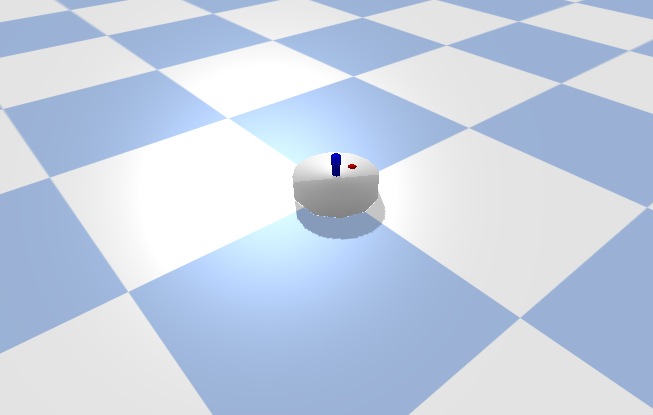
\includegraphics[width=0.8\textwidth]{figures/point_robot.png}
    \caption{The holonomic point robot\\the 2 velocity inputs drive the robot in $x$ and in $y$ direction}%
    \label{subfig:example_point_robot}
    \end{subfigure}%
    \begin{subfigure}{.5\textwidth}
    \centering
    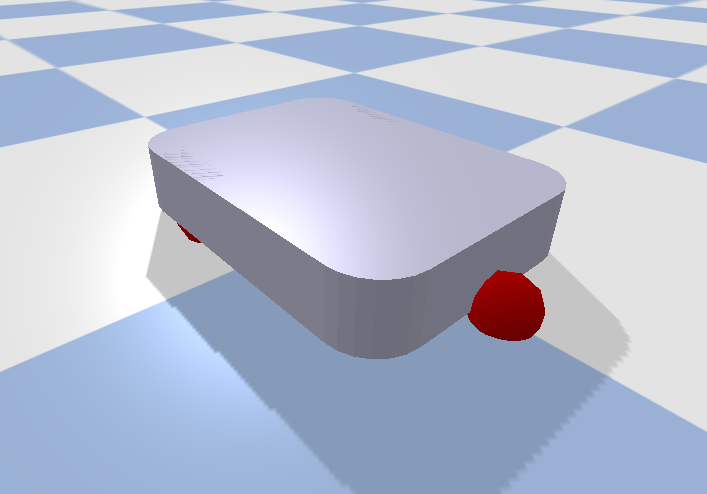
\includegraphics[width=0.8\textwidth]{figures/boxer_robot.png}
    \caption{The nonholonomic boxer robot\\the first velocity input drives the robot forward/backward\\the second rotates the robot}%
    \label{subfig:example_boxer_robot}
    \end{subfigure}%
    \caption{Robots used for testing the proposed method}%
    \label{fig:example_robots}
\end{figure}

\begin{figure}[H]
    \centering
    \begin{subfigure}{.5\textwidth}
    \centering
    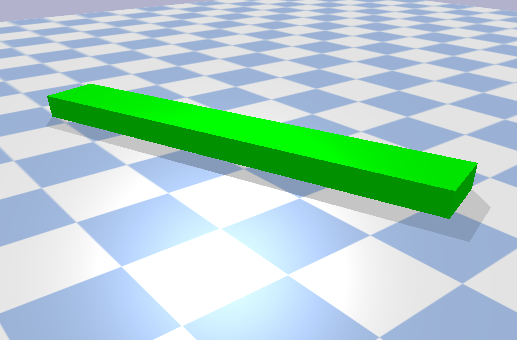
\includegraphics[width=0.8\textwidth]{figures/box_object.png}
    \caption{A box object}
    \end{subfigure}%
    \begin{subfigure}{.5\textwidth}
    \centering
    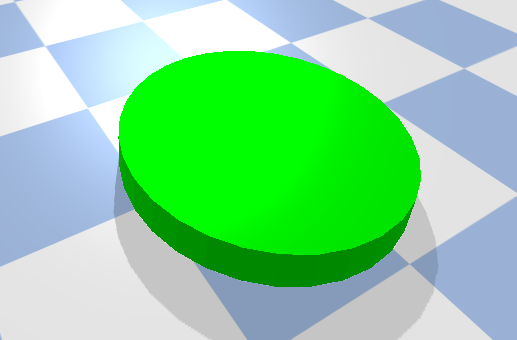
\includegraphics[width=0.8\textwidth]{figures/cylinder_object.png}
    \caption{A cylinder object}
    \end{subfigure}%
    \caption{Various objects in the robot environment}%
    \label{fig:example_objects}
\end{figure}

For complete environments with accompanying tasks, see~\cref{chap:results}.\bs

\subsection{Challenges}%
\label{subsection:problems_with_task_planning}
Finding a solution to a task as defined in \cref{subsec:task}, inside a robot environment defined in \cref{sec:problem_description} bears some challenges. In this section, the main challenge is highlighted and other subchallenges are introduced. Finding a solution requires overcoming the main and subchallenges. Before listing the challenges that this thesis will take on, a challenge is presented that serves to show the difficulty of finding an optimal solution to a task.\bs

\todo[inline]{Martijn: I would remove this whole paragraph. It doesn't clarify much and doesn't convince me that you really know what it means. Gijs: Improve, because I think this paragraph is the thing that actually explainst how difficult the problem is..}
Assuming the task has at least one object to place at a target state (exclude purely \ac{NAMO} problems) \todo[inline]{Martijn: wht is a purely NAMO probelm?}, finding an optimal solution to a task is \ac{NP-hard} since, it can be reduced to the piano mover's problem which is known to be \ac{NP-hard}~\cite{reif_motion_1985}.\\Problems in class P have a solution which can be found in polynomial time, problems in \ac{NP} are problems for which a solution cannot found in polynomial time. For problems in \ac{NP}, when provided with a solution, verifying that the solution is indeed a valid solution can be done in polynomial time. \ac{NP-hard} problems are a class of problems which are at least as hard as the hardest problems in \ac{NP}. Problems that are \ac{NP-hard} do not have to be elements of NP. They may not even be decidable~\cite{pokharel_computational_2020}. This thesis or other recent studies in the references do not attempt to find an optimal solution. Instead, they provide a solution whilst guaranteeing properties such as near-optimality or probabilistic completeness.\bs

Finding a solution to a task requires a search in the \textit{joint configuration space} which comes with 2 problems to tackle. Before investigating a problem, let's investigate how to construct a joint configuration space which is created by augmenting the robot's configuration space with the configuration space of every object. For example, if the configuration space for both robot and objects consist of position $x$, $y$ and orientation $\theta$ around the $z$ axis, then the joint configuration space is $3n$-dimensional, where $n$ is the number of objects including the robot. The joint configuration space's dimensionality grows linearly, meaning the joint configuration space grows exponentially in the number of objects, which is an explosion in the number of possible combinations the environment can be in, the enormity of the joint configuration space is the root of the main challenge.\bs

\todo[inline]{Martijn, "consider a blocked" :strange sentence after the comma}
Unspecified target positions are a fine example of the curse of dimensionality, consider a blocked corridor. The object needs to be pushed to free the path but the target location of this object is unspecified, as long as the robot can drive through the corridor unhindered. A solution is, the robot drives to the object, pushes the object, and then drives through the corridor. The push action influences the free space where the robot has to drive in when the push action was completed. Even sampling-based search algorithms cannot computationally find a path between a start en target state in joint configuration space in reasonable time (orders of magnitude slower than real-time). Only by leveraging simplifications of the joint configuration space a search can be performed, such as discretization~\cite{sabbaghnovin_optimal_2016}, factorization~\cite{vega-brown_asymptotically_2020} or a heuristic function combined with a time horizon~\cite{sabbaghnovin_optimal_2016}. Such techniques prevent searching in configurations relatively far from the current configuration, while optimality guarantees can be given and real-time implementations have been shown.\bs
\todo[inline]{Martijn: There is not first, whilst this section starts with second}

\todo[inline]{Martijn: There is not first, whilst this section starts with second}
The second problem is that the joint configuration space is \textit{piecewise-analytic}. Let's elaborate, when the robot drives constraints apply due to e.g.~the robot being nonholonomic. When the robot pushes an object a different set of constraints are applicable, creating 2 different modes of dynamics. A configuration space containing multiple modes of dynamics is a piecewise-analytic configuration space~\cite{vega-brown_asymptotically_2020}. Motion planners have great difficulty crossing the boundary from one mode of dynamics to another.\bs

The main challenge is to find, for a given task, a path from a starting configuration of the environment (the point in the joint configuration space that the environment starts in) to a desired target configuration in the joint configuration space, where all specified objects are at their target state as specified in the task. Whilst finding such a path requires searching an enormous joint configuration space that is piecewise analytic. The proposed solution will essentially avoid searching directly in the joint configuration space and will search in subspaces of the joint configuration space where only a single mode of dynamics is present. Subchallenges that emerge are system identification, control methods, estimating path existence, motion and manipulation planning. These subchallenges will be properly introduced and elaborated on in \cref{chap:hgraph_and_kgraph}.\bs
\todo[inline]{Martijn: iwhat is a "mode of dynamics"? Configuration spaces are typically not connected to "dynamics".}

\section{Report Structure}%
\label{sec:report_structure}
\todo[inline]{Create the report structure when the report structure does not change anymore}



